\documentclass[letter]{report}
\usepackage{graphicx, subfigure, epsfig} 
\oddsidemargin -0.25in 
\textwidth 6.5in 

%\newcommand {\linespace}{\renewcommand{\baselinestretch}{2}}
%\linespace

\begin {document}

\begin{titlepage}
\begin{center}
%\renewcommand{\baselinestretch}{1}
\large \bf
FASTlib Design and Development Manual\\
\normalsize version 0.1\\ 
\large \bf Fundamental Algorithmic and Statistical Tools (FAST) Lab\\
Georgia Institute of Technology\\
Atlanta, GA
\end{center}
\end{titlepage}

\tableofcontents

\chapter {Introduction}

\section {Overview}
FASTlib is a C/C++ library of state-of-the-art numerical and machine
learning methods.  Its primary design goals are to be versatile, easy
to use, and as fast as possible while still avoiding the worst
problems of developing in a low-level language.  Special emphasis is
given to scalable computation, including algorithms for generalized
$N$-body problems \cite{gray_nips2000} and some support for
parallelization.  Library components are designed to be modular,
facilitating their use as subcomputations of other algorithms.
Further, FASTlib aims to permit rapid, distributed development in an
effort to stay up to date with advances in scientific computation.
Its features include:
\begin{enumerate}
\item A collection of machine learning methods in both executable and
  linkable form that can be used for ``out of box'' analysis.
\item High-performance vectors, matrices, trees, and other data
  structures that can be specialized for a given application via
  templating.
\item Many automated tasks for custom storage types, including memory
  management, serialization, and (very soon) printing to XML.
\item A framework to manage and record parameters, timers, and other
  results involved in all levels of modular computation.
\item An array of debugging and unit testing tools that can be
  compiled out but are still fast when left in.
\item Handy Python scripts for compilation, conducting experiments,
  and analysing resutls.
\end{enumerate}

\section {Background and Motivation}
FASTlib was created in response to the presently disorganized state of
machine learning software, in which the best (if not only) available
implementations of cutting-edge algorithms are typically Matlab
scripts or stand-alone C executables.  Neither of these cases is
optimal in the grand scheme of things.  Matlab may make it easy to
adapt the method for use in other applications, but it suffers from
poor efficiency when doing anything other than linear algebra.  On the
other hand, C code is potentially quick but does not often lend itself
to incorporation into larger projects.  Significant adjustment of data
representation may be necessary, especially if one wants to integrate
C and Matlab.  A further complication is the plethora of solutions
algorithm developers have devised for common tasks such as file I/O,
parsing command line parameters, and reporting results.
Incompatibilities regarding these can lead to a frustrating degree of
end-user written go-between code.

Several attempts have been made to mitigate these problems, including
Weka and arguably Matlab itself.  Neither of these, however, are
generally speedy enough to serve today's premier data mining
applications.  Our aim with FASTlib is to meet this demand by
providing high-performance implementations for numerical and machine
learning methods united by an effective, portable, and consistent API.
We link to other libraries when appropriate---for instance, we defer to
BLAS/LAPACK for (dense) linear algebra---but provide wrappers in order
to standardize and simplify use---finding singular values in LAPACK
involves fourteen parameters, while we need only two.  For the most
part, though, FASTlib directly implements methods of interest in an
effort to maximize their efficiency.

\section {Language and Style}
Various reasons motivated our choice of C/C++ for FASTlib:
\begin{itemize}
\item C/C++ is widely used, well understood, and easily accessible.
\item C/C++ compilers offer high-quality compile-time optimization.
\item While we do not make full use of object-oriented programming,
  encapsulation of code in classes leads to better organization than
  is common in C alone.
\item Relatedly, constructs such as templates and inheritance enable a
  greater extent of code reuse than is possible in C alone.
\item C++ permits both abstraction from memory management when
  convenient and fine control over allocation when necessary.
\item Good tools exist for parallelization in C/C++.
\end{itemize}
Unfortunately, improper use of C++ easily results in confusing,
unmaintainable code.  Accordingly, we have enacted library-wide
precautions against some of C++'s common pitfalls.  Notably, we stick
to C's standard library for I/O tasks, we employ only shallow class
hierarchies, and we make frequent use of compiler-optimized debug
checks.  This last point is especially important in machine learning
as it can be difficult to tell whether statistical or typographical
problems are to blame for an algorithm's lack of convergence.

\section{Development Model}
Core tenets of FASTlib include openness and extensibility, but
supporting these can lead to organizational and political dilemmas:
Who owns the code?  How strictly should style be enforced?  Can
contributions be rejected on stylistic or ideological grounds?  How
can we prevent projects from being forked over disagreements related
to the above?  As of this writing, FASTlib's developers are seeking a
software license that can adequately resolve these issues.

In the meantime, we have devised a staged migration path for
incorporating contributed code into FASTlib's offical toolkits.  In
sketch, this path is as follows:
\begin{enumerate}
\item Experimental code is developed in developers' individual user
  directories in the Subversion repository.  Here, developers have no
  chance of hurting others' work if they must make changes to their
  code's organization, but they may still invite others to review or
  assist with their project.
\item Upon reaching a satisfactory degree of functionality, the code
  is moved into a provisional location where it is tested for proper
  behavior and revised to meet FASTlib library API standards.
  Documentation must also be fully fleshed out by this point.
\item After having been reviewed by sufficiently many members of the
  development community, the code joins the other algorithms in
  FASTlib's extended corpus.  This body of toolkits is the final
  destination for most code.
\item Infrequently, it will be necessary to modify FASTlib's core
  components.  These are held to the strictest standards of quality;
  further, they must remain fast and flexible enough to serve
  everyone's needs.
\end{enumerate}

\begin {figure*}[h]
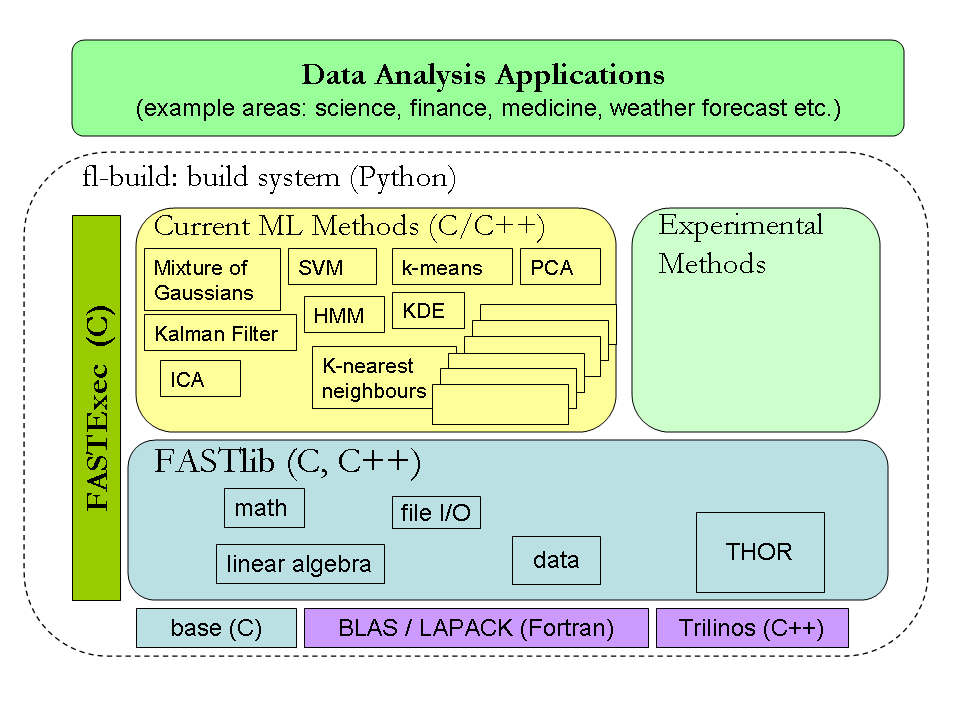
\includegraphics[width=7in,height=5.25in]{Fastlib_Archi.png}
\caption{ Overall Organization of the different components of FASTlib}
\label{fastlib_archi}
\end{figure*}

\section{Why do I want to use FASTlib?} 
Maybe you have an application for an ``out of box'' method, but other
toolkits are too slow.  Maybe you have an algorithm you'd like to
implement in a fast language, but you don't want to reinvent the wheel
regarding data structures and I/O.  Maybe you need to stitch two
methods together in nontrivial ways to do what you want.  Or maybe you
want to make your work available to a community that values fast yet
flexible solutions.  FASTlib is posed to help with all of these
scenarios, so if any of them sound like you, give us a try!

\chapter {Code Development in FASTlib}

\section{Obtaining and Building FASTlib}
FASTlib is intended to be multi-platform, though (without extension)
it relies heavily on the command line; much of the below assumes a
Linux-like interface.  We have tested compilation on the following
systems:
\begin{itemize}
\item Linux: 32-bit x86, 64-bit x86, and Itanium
\item Cygwin (x86 Windows)
\item MacOSX
\end {itemize} 
In order to build FASTlib, you will need the following tools:
\begin {itemize}
\item gcc, g++, and g77 3.4.6; later versions and gfortran should work
\item python 2.2 or later
\item (optional) doxygen and graphviz's dot, for formatted documentation
\end {itemize}

FASTlib is maintained in a Subversion repositoroy at Georgia Tech, but
presently it is available to others in tar-ball format via request.
Let \verb@$FASTLIBPATH@ be the absolute path (i.e.~starting with
\verb@/@) to the directory where you have extracted FASTlib.  You will
need to add \verb@$FASTLIBPATH/script@ to your \verb@$PATH@
environment variable.  This is accomplished differently for different
shells (type \verb@echo $0@ to find out which you are using):
\begin{itemize}
\item For bash or ksh, add to your \verb@.bashrc@ or \verb@.kshrc@
  file (or \verb@.profile@ if the other is absent):
\begin{verbatim}
  export PATH="$FASTLIBPATH/script:$PATH"
\end{verbatim}
\item For csh or tcsh, add to your \verb@.cshrc@ file:
\begin{verbatim}
  setenv PATH "$FASTLIBPATH/script:""$PATH"
\end{verbatim}
\end{itemize}
You will need to close and reopen your terminal to enact the change.
Type \verb@fl-build@ to confirm things are working; this should print
usage information for FASTlib's build system.  Next, try:
\begin{verbatim}
  cd $FASTLIBPATH/u/example
  fl-build main
  ./main --data=fake.arff
\end{verbatim}
This performs 10-fold cross-validation for $k$-nearest-neighbors.  At
the end of the output, you should see
\verb@/kfold/results/p_correct 1.000@; \verb@fake.arff@ was engineered
to be easy.

\section {Code Organization}
The following is subject to some reorganization while FASTlib is still
in its earliest versions, but for now FASTlib is arranged as follows:
\begin{itemize}
\item Core Libraries
  \begin{itemize}
  \item \verb@base/@ - compiler abstractions, debugging, and memory management
  \item \verb@fx/@ - FASTexec client library for managing parameters, timers, and results
  \item \verb@col/@ - templated storage types (dynamic arrays, heaps, etc.)
  \item \verb@data/@ - data set types and utilities
  \item \verb@file/@ - file reading, writing, and tokenization
  \item \verb@math/@ - a collection of math utilities, to be extended as needed
  \item \verb@la/@ - linear algebra routines (mostly a wrapper for BLAS/LAPACK)
  \item \verb@sparse/@ - sparse linear algebra routines (mostly a wrapper for Trilinos)
  \item \verb@trilinos/@ - includes needed for Trilinos
  \item \verb@tree/@ - utilities to build and manage $kd$-trees, among others
  \item \verb@par/@ - rudimentary parallelization utilities
  \item \verb@thor/@ - templated, parallelized algorithm for GNPs
  \item \verb@fastlib/@ - wraps the rest of the library into one convenient include
  \end{itemize}
\item Community-build Code
  \begin {itemize}
  \item \verb@u/@ - the user directory, which contains individual developers' directories
\end {itemize} 
\item  Other
  \begin {itemize}
  \item \verb@script/@ - scripts for compiling code, running experiments, etc.
  \item \verb@util/@ - additional utilities that may assist FASTlib development
  \item \verb@bin/@ - files generated by compilation; \verb@make clean@ deletes this
  \item \verb@bin_keep/@ - compiled binaries that should not be cleaned, such as BLAS/LAPACK
  \end {itemize}
\end{itemize}

\section {Developing your own code using FASTlib}
 
\subsection {Using the build tool}

As stated earlier, building is done via the fl-build tool, which stands for FASTlib build. This tool reads through very short files which just have a list of sources (.cc files), headers (.h files), and other sub-packages it depends on, and produces a Makefile, which it runs automatically.

There are a handful of compilation modes supported by fl-build, specified by the \verb = --mode=mode = parameter. Each mode has a use, and enables certain flags:
\begin{itemize}
\item verbose: tracking the execution of a program when it's infeasible to step through manually. disables optimizations, enables printing of verbosity messages
\item debug: allow best use with gdb for tracking bugs. disables optimization, enables all debug checks, enables highest level of gdb.
\item check (default mode): regular development. enables code optimizations and leaves in debug checks, at a 25% or so penalty. gdb symbols are compiled in but may be inaccurate due to optimizations.
\item fast: timing runs, for the fairest timing comparisons. debug symbols still enabled but may be inaccurate.
\item unsafe: optimizations that might alter correctness, and often will slow the program down.
\item profile: speed profiling. compile with --mode=profile, run your program, and run gprof ./binaryfile | less to see what the bottleneck is. 
\end{itemize}
The command line flags are listed in script/buildsys.py. 

Thus, we could re-build the example, but turn off all debug checks:
\begin{verbatim}
fl-build main --mode=debug
\end{verbatim}
To add custom flags, add \verb= --cflags =. To get increased performance on Pentium 4 and define a macro called \verb= COAGULATE =, you would use:
\begin{verbatim}
fl-build mybinary --mode=fast --cflags="-march=pentium4 -DCOAGULATE"
\end{verbatim}


\subsubsection{Writing build files}

The fl-build tool looks in the current directory for a file called build.py. The build file is executed as straight Python code, with access to a few specific functions defined by the build system, that correspond to "meta build rules". In processing these, the build system recursively pulls build files from other directories and resolves the dependencies. A Makefile is then created in your current directory, which fl-build automatically runs for you.

Here is a sample build rule that will build an executable test compiled from test.cc and test.h, and link it against the fastlib front-end library:
\begin{verbatim}
binrule(
   name = "test",
   sources = ["test.cc"],
   headers = ["test.h"],
   linkables = ["fastlib:fastlib"]
   )
\end{verbatim}
Each string you see is actually processed by the build system, which figures out what you are referring to. If there is no colon ":" character, it looks for a file in the same directory as the build file. If it finds a ":", such as "fastlib:fastlib", it looks in the directory "fastlib" for a rule named "fastlib" -- the left part of the colon is the directory, the right part is the rule name. For example, the full path to the rule for the main executable in \verb= example = would be \verb= ``example:main" =.

Next, suppose you want to create a small reusable library. Taking a look at the build file \verb= u/example/build.py =,
\begin{verbatim}
librule(
    name = "example",              # this line can be safely omitted
          # (since this is u/example, the build system
          # will automatically name it "example" if you omit it -- most
          # other sub-packages will omit the name)
    sources = ["helper.cc"],       # files that must be compiled
    headers = ["helper.h"],        # include files part of the 'lib'
    deplibs = ["fastlib:fastlib"]  # depends on fastlib core
    )

binrule(
    name = "main",                 # the executable name
    sources = ["main.cc"],         # compile main.cc
    headers = [],                  # no extra headers
    linkables = [":example"]       # depends on example in this folder
    )
\end{verbatim}

\subsection{Use of C++}

FASTlib is C++, but only to an extent. If you are familiar with C, you will have no problem. The things we use from C++ is:
\begin{itemize}
\item Templates, for pluggability (used very extensively in THOR)
\item Classes, for coupling data and operations over the data
\item Destructors, to avoid unnecessary clean-up code, and to better support templates 
\end{itemize}
FASTlib mostly avoids inheritance, virtual functions, and operator overloading. It also notably avoids most constructors due to their pickiness about when they are called. Here's an example of what this looks like. In particular, we'll create a multiplication table:
\begin{verbatim}
Matrix mult_table;

mult_table.Init(10, 10); // make it 10 rows by 10 columns

for (index_t i = 0; i < 10; i++) {
  for (index_t j = 0; j < 10; j++) {
    mult_table.set(i, j, i * j);
  }
}
// the matrix does not have to be freed
\end{verbatim}
Some quick notes before we move on. The matrix must be initialized before it is usable, but keep in mind everything is freed by default. Caution -- if you declare a matrix and never initialize it, the program will crash at the end of the function. In debug mode, many FASTlib classes will let you know that this is happening. Next, the \verb= index_t = type is usually an regular int, but is wired through the system to become 64-bit if you tell it to.

\subsection{Copying and Aliasing}

C++ is infamous for its desire to make copies of everything. If you forget to pass a parameter as a constant reference (const Classname\&), everything will be copied, but sometimes, there is just no way to get around of it. By avoiding constructors, we find copying is usually not needed. To avoid accidental copies of your class, put \verb= FORBID_COPY = at the beginning like this:
\begin{verbatim}
class X {
  FORBID_COPY(X);
  ...
}
\end{verbatim}
Sometimes, though, you really need to make copies, or at least things like copies. Many classes support a Copy method to explicitly do so, through the Matrix and Vector.

The Vector and Matrix classes support a concept of aliasing. A vector can be a vector on its own, or it could also point to some column within a matrix; a matrix can also refer to a subset of another matrix's columns. The concept is simple, but there is one caveat: without garbage collection, somebody eventually has to free the memory. Each Vector and Matrix then knows whether it is the owner of the memory it points to, and if it is, it will free the data automatically; otherwise, it is only an alias.

An example is shown here:
\begin{verbatim}
   Matrix original;
   original.Init(5, 5);
   ...
   for (int j = 0; j < 3; ++) {
     Matrix weak_alias;
     weak_alias.Alias(original); // this matrix now aliases the original
     weak_alias.set(j, j, 999.0); // this modifies the original matrix
     // the destructor of weak_alias is called, but the memory is not freed
   }
   Matrix newowner;
   newowner.Own(&original); // newowner
   Matrix copy;
   copy.Copy(original); // a completely new copy 
   original.Destruct(); // newowner is still valid
   original.Init(99, 99);
\end{verbatim}

\subsection{Debugging}

C++, and equally C, can sometimes make it easy to shoot yourself in the foot. To help you avoid this, we made debugging an important part of FASTlib.

The build system by default will enable all checks in the form of \verb= #ifdef DEBUG = (we'll get back to this later). These checks and safeguards, such as bounds checking and memory poisoning, are present in nearly all core FASTlib classes. If you are debugging and find \verb= 0xDEADBEEF, 2146666666, or 0x7FF388AA, or NaN =, it probably means you forgot to initialize something; if you go beyond the end of a Vector, it will let you know. In practice, these have a 20% or so performance penalty -- as a habit, we've found it's just fine to leave these on until you want to run timing experiments. In machine learning code, since you can sometimes generate seemingly good results from garbage data, these types of safeguards are almost essential.

To use debugging yourself, plaster your code with the following:
\begin{itemize}
\item \verb= DEBUG_ASSERT_MSG(condition, format, ...) = - If the condition is false, your program will print the formatted message to stderr and die.
\item \verb= DEBUG_GOT_HERE(3) = - If verbosity is > 3 and verbose-mode is compiled on, it will print the function and line number. 
\end{itemize}
You can safely leave these in at no cost in non debug mode. To set verbosity level to 3.0, you would specify the command line argument: \verb= --debug/verbosity_level=3.0 =.See the Doxygen for base/debug.h for more information.

\subsection{FASTexec - Command-line parameters and experimentation}

We felt it is important that machine learning researchers can run a lot of experiments without too much trouble. Parameter passing is integral to the experimentation process, so we unified these.

The core idea behind the system is that within one run of your program, a hierarchial data store is created. In some ways it is similar to a "Windows registry" except it only has a very brief existence. In fact, it more like an XML document tree, except without attributes, and has a "stateless" output format.

\subsubsection{Basic command-line parameters}

Let's look at a non-trivial example. We're measuring how different strided memory access patterns affect cache performance (something you probably won't care about, but is trivial to code):
\begin{verbatim}
#include "fastlib/fastlib.h"
int main(int argc, char *argv[]) {
  fx_init(argc, argv); // initialize command-line parameters and the data store
  int count = fx_param_int_req( // get a REQUIRED integer parameter
      NULL, // directly from command line (not from a sub module)
      "count"); // called "count", as in --count=num
  int stride = fx_param_int(NULL, "stride", 1); // defaults to stride 1
  double factor = fx_param_double(NULL, "factor", 1.0); // default value 1.0
  
  ArrayList<double> values;
  values.Init(count);

  fx_timer_start(NULL, "strides"); // timers have names
  // Let's see how stride affects cache performance
  for (int s = 0; s < stride; s++) {
    for (int j = s; j < count; j += stride) {
      values[j] = factor * j;
    }
  }
  fx_timer_stop(NULL, "strides");
  fx_format_result(NULL, "success", "%d", 1); // store some result
  fx_done();
}
\end{verbatim}

The useful functions we used were \verb= fx_param_int = (to get an integer), \verb= fx_param_double = (to get a double-precision value), \verb= fx_timer_{start|stop} = to have timers, and \verb= fx_done() = to output the results. I ran this example with the parameters:
\begin{verbatim}
./test --count=10000 --factor=2.0
\end{verbatim}
and the following text resulted:
\begin{verbatim}
<code>
/timers/strides/children/sys 0.000000
/timers/strides/children/user 0.000000
/timers/strides/self/sys 0.000000
/timers/strides/self/user 0.000000
/timers/strides/wall/sec 0.000061
/timers/default/children/sys 0.000000
/timers/default/children/user 0.000000
/timers/default/self/sys 0.000000
/timers/default/self/user 0.000000
/timers/default/wall/sec 0.000354
/params/stride 1
/params/fx/timing 0
/params/debug/print_notify_headers 1
/params/debug/pause_on_nonfatal 0
/params/debug/abort_on_nonfatal 0
/params/debug/print_warnings 1
/params/debug/print_got_heres 1
/params/debug/verbosity_level 1
/params/factor 2.0
/params/count 10000
/results/success 1
/info/rusage/children/nivcsw 0
/info/rusage/children/nvcsw 0
/info/rusage/children/nsignals 0
/info/rusage/children/msgrcv 0
/info/rusage/children/msgsnd 0
/info/rusage/children/oublock 0
/info/rusage/children/inblock 0
/info/rusage/children/nswap 0
/info/rusage/children/isrss 0
/info/rusage/children/idrss 0
/info/rusage/children/ixrss 0
/info/rusage/children/maxrss 0
/info/rusage/children/majflt 0
/info/rusage/children/minflt 0
/info/rusage/children/stime 0.000000
/info/rusage/children/utime 0.000000
/info/rusage/children/WARNING your_OS_might_not_support_all_of_these
/info/rusage/self/nivcsw 1
/info/rusage/self/nvcsw 3
/info/rusage/self/nsignals 0
/info/rusage/self/msgrcv 0
/info/rusage/self/msgsnd 0
/info/rusage/self/oublock 0
/info/rusage/self/inblock 0
/info/rusage/self/nswap 0
/info/rusage/self/isrss 0
/info/rusage/self/idrss 0
/info/rusage/self/ixrss 0
/info/rusage/self/maxrss 0
/info/rusage/self/majflt 0
/info/rusage/self/minflt 393
/info/rusage/self/stime 0.002999
/info/rusage/self/utime 0.002999
/info/rusage/self/WARNING your_OS_might_not_support_all_of_these
/info/system/kernel/build %231%20SMP%20Tue%20Jan%2023%2012%3A49%3A51%20EST%202007
/info/system/kernel/release 2.6.9-42.0.8.ELsmp
/info/system/kernel/name Linux
/info/system/arch/name x86_64
/info/system/node/name shannon.cc.gatech.edu
\end{verbatim}
We admit this is a lot of text, but when you later comb through the results, you can select only the portions you care about. Briefly, each portion of the tree:
\begin{itemize}
\item params/ - Parameters you were called with. Default parameters are explicitly stored in case you later change what the default values are.
\item timers/ - Each timer. There will always be a default timer, which runs between \verb= fx_init = and \verb= fx_done =.
\item results/ - Results that you decided to emit.
\item info/rusage/ - System information related to rusage. See the manpage for getrusage(2).
\item info/system/ - Information on the system run on. See manpage for uname(2). 
\end{itemize}
This output could indeed just be an s-expression, or it could be an attribute-less XML file. We chose this path-value dump format because it is stateless -- i.e. anyone can process it with a little bit of grep. Corruption in the file will only affect it until the next newline.

\subsubsection{Running automated experiments and collecting results}

Running experiments and collecting results is made simpler using FASTexec. After using the FASTexec code to store output variables in the datastore, you can use FASTexec to run multiple experiments. If you type the command:
\begin{verbatim}
fx-run | less
\end{verbatim}
you will see the help screen for fx-run. This program will run your executable with all combinations of the parameters you give it, and save results in a directory called fx that is created in the same directory you run the tests. After that, gather results using fx-csv to make an Excel-compatible comma-separated-values file, or fx-latex to create a properly escaped LaTeX table.

You can try an example with the K-nearest-neighbors classifier example in u/example:
\begin{verbatim}
  cd $FASTLIBPATH/u/example && fl-build main
  fx-run knn_k ./main --knn/k=1,2,3,4,5 --data=../../../../fake.arff
  fx-csv knn_k ./main /params/knn/k /kfold/results/p_correct
  fx-latex knn_k ./main /params/knn/k /kfold/results/p_correct --preview
\end{verbatim}

\subsection{Little gotchas}

\subsubsection{Success and failure}

The \verb= success_t type = in \verb= base/common.h = defines our standard for indicating success or failure. Rather than assuming 1 or 0 or -1 indicates something or other, we explicitly return \verb= SUCCESS_PASS = (succeeded), \verb= SUCCESS_FAIL = (failed), or \verb= SUCCESS_WARN = (something was suboptimal).

\subsubsection{Basic types}

You will notice heavy use of \verb= index_t = (in \verb= base/scale.h =) rather than integers. For practical purposes, \verb= index_t = is a signed integer -- signed so you can loop over >= 0. On 32-bit and 64-bit Intel/AMD machines, this will be 32-bits, which is the fastest int for both systems and is relatively compact. But if you want to operate on datasets larger than a few gigabytes, you can define the \verb= SCALE_LARGE = macro, and these will instantly switch to the largest size your computer can address.

Also, the \verb= base/basic_types.h = file (it will be in bin/ since it is auto-generated) defines standard int16, int32, int64, uint16, uint32, uint64 types.

\subsubsection{Printf versus Streams}

We operate under the assumption that more of our audience is familiar with C I/O than with C++ I/O, especially when it comes to fancy floating-point formatting. The caveat is that printf only works with native types like int, short, long. To print an \verb= index_t =, you use:
\begin{verbatim}
printf("Iteration %"LI"d complete.", some_index_var);   // no special formatting
printf("Iteration %04"LI"d complete.", some_index_var); // with formatting
\end{verbatim}
The LI macro is a string that will have the suitable "l" modifier for \verb= index_t = (see man sprintf for more details). For other types:
\begin {itemize}
\item int16 and uint16: L16
\item int32 and uint32: L32
\item int64 and uint64: L64 
\end{itemize}
Alternately, you can just cast the variable to a native type like (int) (short) or (long), if you want to be lazy.


\chapter {Complete code development walkthrough - Dual-Tree k-NN}
This chapter is intended for people who have read the FASTlib Tutorial and successfully compiled and run the example code. You should also understand how a dual-tree all nearest neighbors algorithm works, since this is assumed. 

This should help you get started on understanding the basic features of the library. For complete documentation, please see the Doxygen file. 

\section{Walkthrough} 
\subsection{build.py} 
The build.py file is a necessary part of any FASTlib directory. It tells the fl-build script how to compile your code and link to the rest of the library. Essentially, the build.py functions like a Makefile, but is much easier to understand and write. 

There are two important kinds of entry in build.py files: binrules and librules. The distinction between these is that binrules create stand-alone executables (somewhere in their code is the main function) while librules are for code used in linking (no main). It is usually a good idea for the bulk of your project to be compiled with a librule, linked to by a simiple binrule in the same build.py: 

\subsection{Librule} 
\begin{verbatim}
 librule(
   name = "allnn",
   sources = ["allnn.cc"],
   headers = ["allnn.h"],
   deplibs = ["fastlib:fastlib"],
   tests = ["allnn_test.cc"]
 )
\end{verbatim}
name - the name of the library being created. If this line is omitted, fl-build will use the name of the directory as a default.\\ 
sources - The .c or .cc files necessary. This line can be omitted if there are none.\\ 
headers - The .h files necessary. This line can also be omitted if there are none.\\ 
deplibs - Other libraries linked to by the current one. The name before the colon is the directory within fastlib that contains the library, the name after the colon is the name of the library itself.  :\$LIBNAME indicates that the library is in the same directory as the build.py file. 
tests - A file containing unit tests. If this line is in the librule, you can compile the unit tests with fl-build allnn\_test. 
\subsection{Binrule}

\begin{verbatim} 
 binrule(
   name = "allnn_main",
   sources = "allnn_main.cc",
   headers = "allnn_main.h",
   deplibs = [":allnn"]
 )
\end{verbatim}
The tags are similar as above. Running "fl-build allnn\_main" will create an executable called "allnn\_main". 

\subsection{allnn\_main.cc} 
Our main file contains only the main function. In general, FASTlib code should have very simple main functions. Our main function reads in the command line arguments, loads the data, and saves the results. All of the computation is done by an AllNN object, defined in allnn.h. 

\section{FASTexec} 
See FASTexec Tutorial for a more detailed discussion of FASTexec. 
FASTlib code starts by calling: 

\begin {verbatim} fx_init(argc, argv);\end{verbatim}
which initializes the FASTexec system. It must be accompanied by: 

\begin{verbatim} fx_done(argc, argv);\end{verbatim}
at the end of the main function. 

\section {Reading and writing data} 
Our function determines the files containing the query and reference data. We accomplish this with: 
\begin{verbatim}
const char* queries_file_name = fx_param_str_req(NULL, "q");
Matrix queries; 
data::Load(queries_file_name, &queries);
end{verbatim}
The only other parameters our program reads are a boolean: 
\begin{verbatim}
int do_naive = fx_param_bool(NULL, "do_naive", 0);
\end{verbatim}
and the output filename: 
\begin{verbatim}
const char* output_filename = fx_param_str(NULL, "output_filename", "output.csv");
\end{verbatim}
In general, data can be read in from the command line using 
\begin{verbatim}
fx_param_$TYPE_req(module, "name");
\end{verbatim}
for required parameters (the program will terminate with an error if it is not specified). Alternatively, one can specify a default value with: 
\begin{verbatim}
fx_param_$TYPE(module, "name", $DEFAULT_VALUE);
\end{verbatim}
In both cases, the parameter is given on the command line as 
\begin{verbatim}
--name=$VALUE"
\end{verbatim}

\section{Modules} 
The first argument to each of these functions indicates a module. Modules contain parameters, results, and timing information for various portions of the program. For a detailed explanation of modules, consult the FASTexec Tutorial. 

For this code, we only utilize a few modules. When NULL is passed as a module, it indicates the root module of FASTexec. So, the line: 
\begin{verbatim}
const char* output_filename = fx_param_str(NULL, "output_filename", "output.csv");
\end{verbatim}
indicates that \begin{verbatim}--output_filename="some_file.csv"\end{verbatim} will appear on the command line (i.e. specified in the root module's /params folder), or else "output.csv" will be used as the default. 

We also create a module for our AllNN object. The line: 
\begin{verbatim}fx_submodule(NULL, "allnn", "allnn_module");\end{verbatim}
creates a new module called "allnn\_module", copies all parameters
stored under allnn to this module, and places the entire thing under
the root directory (NULL).

\section{Timers} 
Timers are also handled by FASTexec. They are stored in the /timers section of a module. We can start a timer with: 
\begin{verbatim}
fx_timer_start(allnn_module, "dual_tree_computation");
\end{verbatim}
and stop it with 
\begin{verbatim}
fx_timer_stop(allnn_module, "dual_tree_computation");
\end{verbatim}

These timers will print as a part of the final output of the program, and are suitable for parsing with the fx-run commands. 
Timers, modules, and command line parameters can be accessed from any part of the program, not just main. 

\section{Development Walkthrough}
You are developing code. What to do, step by step: 

Step 0: You should have read the FASTlib tutorial and successfully compiled and run the example.\\ 

Step 1: Your code needs a home. You will work on it in your user directory, i.e.: u/plato/allnn\\

Step 2: You need a build.py file, which tells fl-build what to do to compile your work. It is the equivalent of a Makefile, but a bit easier to understand. 

There are two important kinds of entry in build.py files: binrules and librules. The distinction between these is that binrules create stand-alone executables (somewhere in their code is the main function) while librules are for code used in linking (no main). It is usually a good idea for the bulk of your project to be compiled with a librule, linked to by a simiple binrule in the same build.py: 

\begin{verbatim}
 librule(
   name = "allnn",
   sources = ["allnn.cc"],
   headers = ["allnn.h"],
   deplibs = ["fastlib:fastlib"],
   tests = ["allnn_test.cc"]
 )

 binrule(
   name = "allnn_main",
   sources = "allnn_main.cc",
   headers = "allnn_main.h",
   deplibs = [":allnn"]
 )
\end{verbatim}

Note that "tests" in the librule allows you to compile your unit tests with "fl-build allnn\_test". 

Step 3: Now we need to start writing the code. We will start with allnn\_main.cc by incluidng allnn.h at the top and writing a main function: 

\begin{verbatim}
 #include "allnn.h"
 int main(int argc, char *argv[]) {
   fx_init(argc, argv);
   ...
   fx_done();
   return 0;
 }
\end{verbatim}

FASTlib main functions should always begin and end by initializing and finalizing fx, or FASTexec, which manages command line input among other things. 

In our particular project, the first logical thing to do is to load the data. We need to get the input file names out of the command line arguments and then to use a library function that reads matrices. 

\begin{verbatim}
 const char *q_filename = fx_param_str_req(NULL, "queries");
 const char *r_filename = fx_param_str_req(NULL, "references");
 Matrix q;
 Matrix r;
 data::Load(q_filename, &q);
 data::Load(r_filename, &r);
\end{verbatim}

We organize all of our project's tasks into a class called AllNN. After declaring an object of this class, we initialize it with the two data sets and a submodule, which serves to pass it its own parameters from the command line. 

\begin{verbatim}
 struct datanode *allnn_mod = fx_submodule(NULL, "allnn", "allnn_mod");
 AllNN allnn;
 allnn.Init(q, r, allnn_mod);
\end{verbatim}
We must declare a local variable to receive the results of computation. 
\begin{verbatim}
 ArrayList<index_t> results;
 allnn.ComputeNeighbors(&results);
\end{verbatim}
We emit result by printing to a file. 
\begin{verbatim}
 const char *o_filename = fx_param_str(NULL, "out", "out.csv");
 FILE* o_file = fopen(o_filename, "w");
 ot::Print(results, o_file);
\end{verbatim}

Step 4: Moving to allnn.h, the first thing to do include the rest of FASTlib within appropriate inclusion guards: 

\begin{verbatim}
 #ifndef ALLNN_H
 #define ALLNN_H
 #include "fastlib/fastlib.h"
 ...
 #endif
\end{verbatim}

Make sure you include "fastlib/fastlib.h" as opposed to "fastlib.h" so the complier can properly find the file.\\ 

Step n: Write your unit tests. 

NOTE: This chapter still need more work.

\chapter {Examples of some common tasks - FASTlib Cookbook}

\chapter {Code Style Suggestion for developers}
The coding style suggestions in this chapter stem from our own development expereince and the style used to develop FASTlib. It is recommended that you use the suggestions herein for your code development if you would like to contribute your code to be part of the standard FASTlib distribution. You could also choose to skip this chapter.

\chapter {Beyond this Document} 
\end{document}
